\documentclass[cal1spr16Lectures.tex]{subfiles}
%\AtBeginSubsection{
%	\begin{frame}[allowframebreaks]{}
%	\begin{multicols}{2}
%	\tableofcontents[currentsubsection]
%	\end{multicols}
%	\end{frame}
%	}
	
\begin{document}

%\section[Week 5]{Week 5: 15-19 February}

% % %
\subsubsection{\bf Monday 15 February}
\begin{frame}[allowframebreaks]{Mon 15 Feb}
\begin{itemize}\footnotesize
\item Expect Exam back on Thursday.
\item Quizzes: 
\begin{itemize}\footnotesize
	\item Include drill instructor and time.
	\item Don't turn in the Quiz sheet with your work.
	\item Drill Exercise Tues 16 Feb and Quiz 4 Thurs 18 Feb.
\end{itemize}
\framebreak
\item  Announcement: 

\alert{A student in this class requires a note-taker. If you are willing to upload your notes and plan to attend class on a REGULAR basis, please sign up via the CEA Online Services on the Center for Educational Access (CEA) website \url{http://cea.uark.edu}. On the CEA Online Services login screen, click on ``Sign Up as a Note-taker". At the end of the semester you will receive verification of 48 community service hours OR a \$50 gift card for providing class notes. All interested students are encouraged to sign up; preference may be given to volunteers seeking community service in an effort engage U of A students in community service opportunities. Please contact the Center for Educational Access at ceanotes@uark.edu if you have any questions.}

\end{itemize}
\end{frame}

% % %
\subsection[3.2 Graphing the Derivative]{\S 3.2 Graphing the Derivative}
% % %

% % %
\begin{frame}{\S 3.2 Graphing the Derivative}
Recall: The graph of the derivative is essentially the graph of the collection of slopes of the tangent lines of a graph.  If you just have a graph (without an equation for the graph), the best you can do is approximate the graph of the derivative.
\end{frame}

% % %
\begin{frame}{}{}
%\vspace{1pc}
{\bf Simple Checklist:} 
\begin{itemize}
\item[1. ] Note where $f'(x)=0$.
\item[2. ] Note where $f'(x)>0$. 
\begin{que} What does this look like? \end{que}
\item[3. ] Note where $f'(x)<0$.
\begin{que} What does this look like? \end{que}
\end{itemize}
\end{frame}

% % %
\begin{frame}{}
\begin{ex}
Given the graph of $g(x)$, sketch the graph of $g'(x)$.

\begin{center}
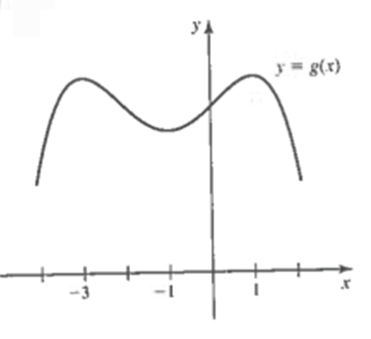
\includegraphics[scale=0.9]{pictures/Ch3Sect2new1}
\end{center}
\end{ex}
\end{frame}

% % %
\begin{frame}
\begin{center}
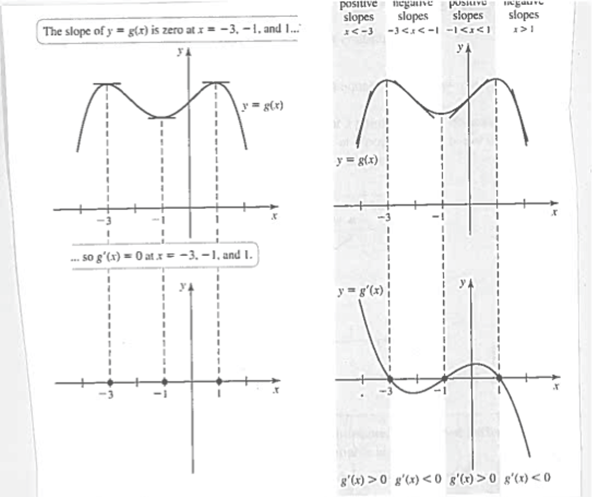
\includegraphics[scale=0.9]{pictures/Ch3Sect2new2}
\end{center}
\end{frame}

% % %
\begin{frame}
\begin{ex}[With Asymptopes]
Given the graph of $f(x)$, sketch the graph of $f'(x)$.

\begin{center}
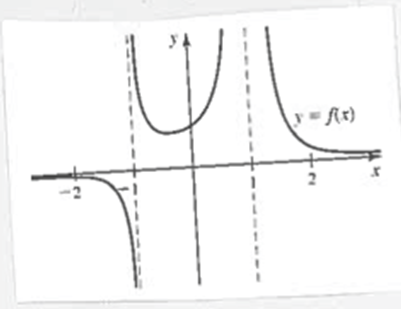
\includegraphics[scale=1]{pictures/Ch3Sect2new3}
\end{center}
\end{ex}
\end{frame}

% % %
\begin{frame}
\begin{center}
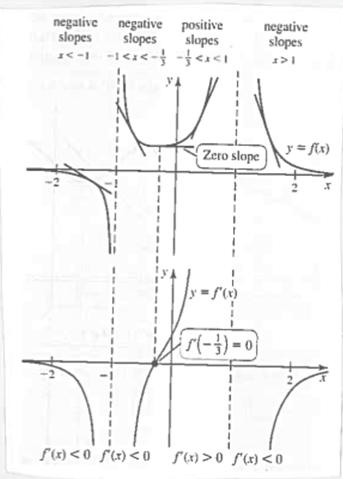
\includegraphics[scale=1]{pictures/Ch3Sect2new4}
\end{center}
\end{frame}

% % %
\begin{frame}
Recall the relationship between differentiability and continuity.
\begin{exe}
If a function $g$ is not continuous at $x=a$, then $g$
\begin{itemize}
\item[A. ] must be undefined at $x=a$.
\item[B. ] is not differentiable at $x=a$.
\item[C. ] has an asymptote at $x=a$.
\item[D. ] all of the above.
\item[E. ] A. and B. only.
\end{itemize}
\end{exe}
\end{frame}

% % %
\subsubsection{Book Problems}
% % %

% % %
\begin{frame}{}
\begin{block}{3.2 Book Problems} 5-14 \end{block} 
\end{frame}

% % % 
\subsection[3.3 Rules of Differentiation]{\S 3.3 Rules of Differentiation}
% % %

% % %
\begin{frame}{\S 3.3 Rules of Differentiation}
Recall the definition of the derivative:
\[f^{\prime}(x)=\lim_{h \to 0} \frac{f(x+h)-f(x)}{h}\]
(as a function of $x$, i.e., a formula).

And, for any particular point $a$, we have 
\[f^{\prime}(a)=\lim_{x \to a} \frac{f(x)-f(a)}{x-a}.\]
\end{frame}

% % %
\subsubsection{Constant Functions}
% % %

% % %
\begin{frame}{\small Constant Functions}\footnotesize
The constant function $f(x)=c$ is a horizontal line with a slope of 0 at every point.  This is consistent with the definition of the derivative:
\begin{align*}
f^{\prime}(x)&=\lim_{h \to 0} \frac{f(x+h)-f(x)}{h} \\
 &=\lim_{h \to 0} \frac{c-c}{h} \\[0.5pc]
 &=\lim_{h \to 0} 0 = 0.
\end{align*}
Therefore, for constant functions, \alert{$\frac{d}{dx}c=0$}.
\end{frame}

% % %
\subsubsection{Power Rule}
% % %

% % %
\begin{frame}{\small Power Rule}{}
{\bf Fact:} For any positive integer $n$, we can factor
\[x^n-a^n=(x-a)(x^{n-1}+x^{n-2}a+\cdots+xa^{n-2}+a^{n-1}).\]

For example, when $n=2$, we get
\[x^2-a^2=(x-a)(x+a),\]
which is the difference of squares formula.
\end{frame}

% % %
\begin{frame}{\small Power Rule, cont.}\footnotesize
Suppose $f(x)=x^n$ where $n$ is a positive integer.  Then at a point $a$,
\begin{align*}
f^{\prime}(a) &= \lim_{x \to a} \frac{f(x)-f(a)}{x-a} = \lim_{x \to a} \frac{x^n - a^n}{x-a} \\[0.25pc]
&= \lim_{x \to a} \frac{(x-a)(x^{n-1}+x^{n-2}a + \dots + xa^{n-2}+a^{n-1})}{x-a} \\[0.25pc]
&= (a^{n-1}+a^{n-2}\cdot a + \dots + a \cdot a^{n-2} + a^{n-1}) = n a^{n-1}. 
\end{align*}
Using the formula for the derivative as a function of $x$, one can show \alert{$\frac{d}{dx} (x^n)= nx^{n-1}$}.
\end{frame}

% % %
\subsubsection{Constant Multiple Rule}
% % %

% % %
\begin{frame}{\small Constant Multiple Rule}
Consider a function of the form $cf(x)$, where $c$ is a constant.  Just like with limits, we can factor out the constant: 
\begin{align*}
\frac{d}{dx}[cf(x)] &= \lim_{h \to 0} \frac{cf(x+h)-cf(x)}{h} \\
&= \lim_{h \to 0} \frac{c[f(x+h)-f(x)]}{h} = c\lim_{h \to 0} \frac{f(x+h)-f(x)}{h} \\[0.25pc]
&= cf^{\prime}(x)
\end{align*}
Therefore, \alert{$\frac{d}{dx}[cf(x)]=cf^{\prime}(x)$}.
\end{frame}

% % %
\subsubsection{Sum Rule}
% % %

% % %
\begin{frame}{\small Sum Rule}
Sums of functions also behave under the same limit laws when we differentiate:
\begin{align*}
\frac{d}{dx}[f(x)+g(x)] &= \lim_{h \to 0} \frac{[f(x+h)+g(x+h)]-[f(x)+g(x)]}{h} \\
&= \lim_{h \to 0} \left[\frac{[f(x+h)-f(x)]}{h}+\frac{[g(x+h)-g(x)]}{h}\right] \\[0.25pc]
&= \lim_{h \to 0} \frac{f(x+h)-f(x)}{h}+ \lim_{h \to 0}\frac{g(x+h)-g(x)}{h} \\[0.25pc]
&= f^{\prime}(x)+g^{\prime}(x)
\end{align*}
\end{frame}

% % %
\begin{frame}{}
So if $f$ and $g$ are differentiable at $x$,
\[\alert{\frac{d}{dx}[f(x)+g(x)]=f^{\prime}(x)+g^{\prime}(x)}.\]
The Sum Rule can be generalized for more than two functions to include $n$ functions.

\vspace{1pc}
{\bf Note:}  Using the Sum Rule and the Constant Multiple Rule produces the Difference Rule:
\[\alert{\frac{d}{dx}[f(x)-g(x)]=f^{\prime}(x)-g^{\prime}(x)}.\]
\end{frame}

% % %
\begin{frame}
\begin{exe}Using the differentiation rules we have discussed, calculate the derivatives of the following functions.  Note which rule(s) you are using.
\begin{itemize}
\item[1.] $y=x^5$
\item[2.] $y=4x^3-2x^2$
\item[3.] $y=-1500$
\item[4.] $y=3x^3-2x+4$
\end{itemize}
\end{exe}
\end{frame}

% % %
\subsubsection{Exponential Functions}
% % %

% % %
\begin{frame}{\small Exponential Functions}\footnotesize
Let $f(x)=b^x$, where $b>0$, $b \neq 1$.  To differentiate at $0$, we write
\[f^{\prime}(0)=\lim_{x \to 0}\frac{f(x)-f(0)}{x-0}=\lim_{x \to 0} \frac{b^x-b^0}{x}=
\lim_{x \to 0} \frac{b^x-1}{x}.\]

\vspace{1pc}
It is not obvious what this limit should be.  However, consider the cases $b=2$ and $b=3$.  By constructing a table of values, we can see that 
\[\lim_{x \to 0} \frac{2^x-1}{x} \approx 0.693 \quad \text{and}\quad \lim_{x \to 0} \frac{3^x-1}{x} \approx 1.099.\]
\end{frame}

% % %
\begin{frame}\footnotesize
So, $f^{\prime}(0)<1$ when $b=2$ and $f^{\prime}(0)>1$ when $b=3$.  As it turns out, there is a particular number $b$, with $2<b<3$, whose graph has a tangent line with slope 1 at $x=0$.  In other words, such a number $b$ has the property that 
\[\lim_{x \to 0} \frac{b^x-1}{x}=1.\]
\begin{que}What number is it? \end{que}
{\bf Answer:} This number is $e=2.718281828459 \dots$ (known as the Euler number).  The function $f(x)=e^x$ is called the \alert{\bf natural exponential function}.
\end{frame}

% % % 
\begin{frame}\footnotesize
Now, using  $\displaystyle\lim_{x \to 0} \frac{e^x-1}{x}=1$, we can find the formula for $\frac{d}{dx}(e^x)$:
\begin{align*}
\alert{\frac{d}{dx}(e^x)} &= \lim_{h \to 0} \frac{e^{x+h}-e^x}{h} \\[0.25pc]
 &= \lim_{h \to 0}\frac{e^x \cdot e^h -e^x}{h} \\[0.25pc]
 &= \lim_{h\to 0}\frac{e^x(e^h-1)}{h} \\[0.25pc]
 &=e^x \left(\lim_{h \to 0} \frac{e^h-1}{h}\right) \\[0.25pc]
  &= e^x \cdot 1 = \alert{e^x}
\end{align*}
\end{frame}

\end{document}